\chapter*{Introducción}

En un sólido cristalino los átomos se distribuyen de forma espacialmente regular constituyendo una red  periódica. Los electrones en la red pueden clasificarse en dos categorías enteramente diferenciadas: aquellos que están fijos a los orbitales internos de los átomos de la red; y aquellos que, por encontrarse en los orbitales más externos, pueden desligarse de dichos orbitales, y que forman lo que se conoce como estructura de bandas. 

Como un ejemplo de un fenómeno físico, de gran interés asociado a estructura de la red, puede comentarse que la conductividad eléctrica de un sólido está determinada por la respuesta de los electrones móviles de la red a los campos eléctricos externos \cite{kittel}. 

\begin{figure}[h]
    \centering
\includegraphics[scale=0.5]{./imagenes/NA-CL-Halit-Kristalle.jpg}
    \caption{Cristales de Halita (sal).}
    \label{fig:NACL_1}
\end{figure}

\begin{figure}[h]
    \centering
    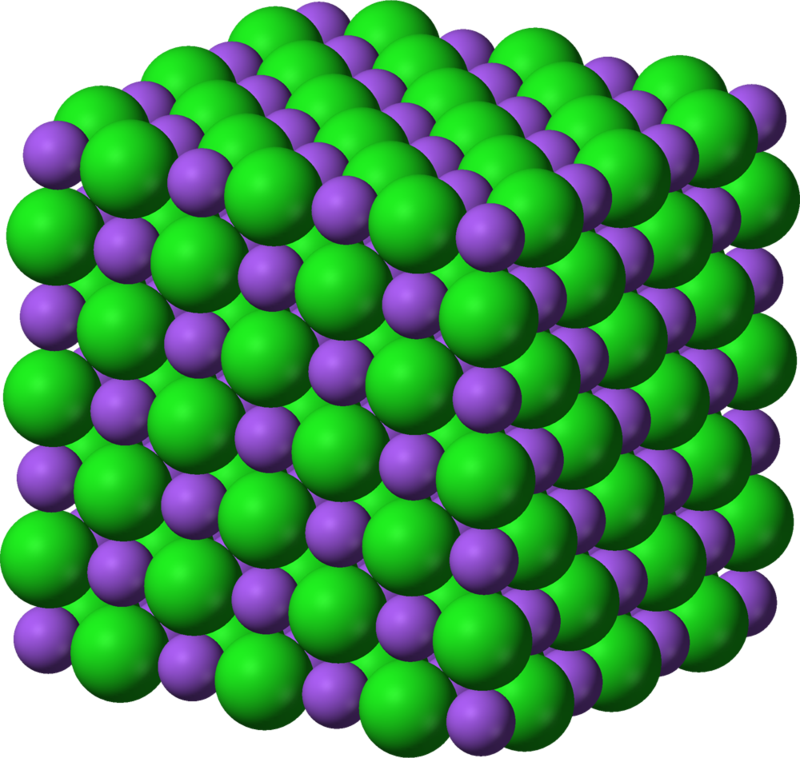
\includegraphics[scale=0.2]{./imagenes/NA-CL-Sodium-chloride-3D-ionic.png}
    \caption{Los átomos de sodio y cloro en su ordenamiento espacial}
    \label{fig:NACL_2}
\end{figure}


El problema de movilidad de los electrones en el sólido es, en principio, un problema de muchos cuerpos \cite{Fetter} \cite{kit_esteroides} . La dinámica de los electrones inmersos en la red debe tomar en cuenta no solo la interacción de los electrones con el potencial de los iones, sino también las interacciones electrón-electrón. El Hamiltoniano del i-ésimo electrón móvil de la red es: 

\begin{equation}
\mathbf{H}=\mathbf{T}_i+\sum_{j\neq{}i}\,V(r_{ij})+\sum_{j}\,U(r_{ij})\,,
\end{equation}
donde $\mathbf{T}_i$ es el operador de energía cinética del electrón, $V(r_{ij})$ el potencial de interacción entre el i-ésimo y el j-ésimo electrón y $U(r_{ij})$ el potencial de interacción con el j-ésimo núcleo en la red \cite{Fetter}. El tratamiento de la teoría en estos términos es sumamente complejo, y es por ello que se recurre a aproximaciones que han resultado sumamente exitosas.

En la aproximación de un solo electrón, todas las interacciones sobre este se representan por un solo potencial efectivo $U(\mathbf{r})$, cuando se pretende modelar un cristal perfectamente periódico el potencial efectivo resulta ser periódico \cite{ashc}. 
En términos cualitativos, se espera que, en el caso unidimensional homonuclear, de interés para este trabajo, el potencial cristalino típico tenga la forma que se muestra en la figura 
\ref{fig:periodic_potential}.
\begin{figure}[h]
    \centering
    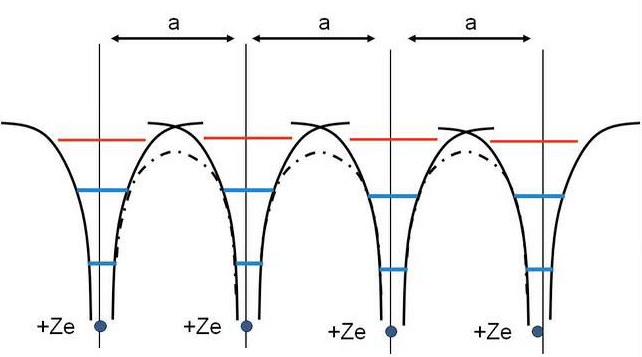
\includegraphics[scale=.5]{./imagenes/Periodic_Potential_1.png}
    \caption{Potencial periódico unidimensional}
    \label{fig:periodic_potential}
\end{figure}

La dinámica de electrones en redes periódicas fue extensamente estudiada por Bloch y Floquet, debido a esta razón histórica, los electrones en la red se llaman electrones de Bloch.

Expresado en términos modernos, el resultado fundamental de Bloch se expresa diciendo que la función de onda electrónica en una red periódica, porta una representación del grupo de traslaciones, es decir,
\begin{equation}
    \psi(x)=e^{ikx}\,u(x)\,,
\end{equation}
donde el número de onda ($k=2\pi/a$) se escoge dentro de la primera zona de Brillouin y $u$ es una función periódica de período $a$.

Otra de las aproximaciones que se utiliza, es la denominada aproximación de \textit{Tight Binding} \cite{ashc}, relacionada con el método de combinaciones lineales de orbitales atómicos que se utiliza ampliamente en química computacional, en particular en los denominados cálculos {\it{ab initio}}. El método consiste en utilizar una base del espacio de estados (lo que no implica resolver las ecuaciones del problema) para estudiar la estructura de bandas. El método de enlace fuerte lleva a una expresión altamente no lineal para la energía cinética del electrón en la red (relación de dispersión) $E=E(k)$ que constituye uno de los objetos fundamentales de este trabajo.

El fenómeno de \textit{Localización Dinámica} fue sugerido por el trabajo de Dunlap y  Kenkre en 1986 \cite{Dunlap}. Cuando un electrón en una red de \textit{Tight Binding} es sometido a un potencial eléctrico sinusoidal su posición inicial será restaurada en periodos del potencial aplicado. También se encuentra que el desplazamiento cuadrático promedio del electrón estará acotado y tendrá forma sinusoidal. Cuando el electrón presenta este comportamiento en las condiciones expuestas se dice que presenta localización dinámica. Para poder observar las oscilaciones en localización dinámica se debe cumplir la condición $\omega\tau>1$,donde $\tau$ es el tiempo libre medio del electrón. Para este proyecto de grado, se quiere estudiar el comportamiento dinámico de la partícula cuando el campo  eléctrico aplicado es inhomogéneo.

En la última década del siglo pasado, se hizo posible obtener cristales cuya distancia entre planos es del orden de $10$ \AA, cuando la distancia usual es de aproximadamente $1$ \AA$\,$   \cite{wannier2}, adicionalmente, ha sido posible disminuir de manera muy importante la cantidad de impurezas. En estos cristales, el tiempo de tránsito medio del electrón (antes de experimentar una dispersión) es mucho más largo que en un cristal convencional. Como consecuencia de estos avances técnicos, se ha hecho posible observar fenómenos que antes permanecían ocultos a la detección, como  por ejemplo, las oscilaciones de Bloch. Esto ha revivido el interés por los estudios teóricos de estos hechos lo que, sin duda, es una importante justificación para este trabajo. 

Matínez et al.\cite{mart2014} presentan un estudio semiclásico del movimiento de un electrón en una red cristalina, cuando sobre este actúa un potencial no homogéneo rápidamente oscilante, obteniendo una fórmula para el hamiltoniano efectivo de la dinámica lenta del sistema. En el 2017, Martínez y colaboradores retoman el estudio del mismo tipo de sistemas llevando el análisis a una formulación cuántica completa  \cite{martinez2017}

El objetivo general de este trabajo consiste en modelar la dinámica de un electrón en la red, cuando sobre él actúan campos externos inhomogéneos y rápidamente oscilantes; utilizando como método de estudio el modelo de \textit{Tight Binding}. 

En particular, se pretende modelar la dinámica del electrón en una red unidimensional, perfectamente periódica, homonuclear, sin impurezas, restringiendo al electrón a mantenerse dentro de una sola banda, es decir, sin considerar transiciones de banda. 

En vista de que el sustrato en el que se encuentra el electrón es una red (potencial periódico), se utilizan la teoría de Floquet y el teorema de Bloch. En el trabajo se buscan potenciales efectivos y se hacen tanto estudios semiclásicos como cuánticos logrando reproducir los resultados de Martínez et al. (2014) \cite{mart2014} y  Martínez et al. (2017), y estudiando la dinámica de partículas en campos no homogéneos.

En el enfoque semiclásico se utiliza el método de Kapitza para partículas clásicas con perturbaciones externas rápidamente oscilantes, y se aplica al electrón en la red. Kapitza estudió partículas clásicas en presencia de campos rápidamente oscilantes, concluyendo que el sistema se puede modelar separando los movimientos de la partícula en uno rápido y otro lento. Y, a partir de allí encuentra el potencial efectivo.

Se obtiene la forma de la aceleración efectiva del electrón dentro del cristal, y, probando perturbaciones específicas se puede hallar el potencial efectivo y así hacer un modelo para la dinámica del electrón bajo la influencia de  cualquier potencial externo, rápidamente oscilante o no. 

En interesante hacer el estudio cuántico por su exactitud. En particular, se utilizara un enfoque perturbativo, basado en los trabajos de Floquet- Magnus y el método de Maricq.  Se estudia el efecto de los potenciales externos sobre un electrón en una red de enlace fuerte. Este es un método aproximado, la expansión de Floquet-Magnus aproxima el Hamiltoniano efectivo del electrón en la red en presencia de la perturbación. Esta aproximación se hace hasta cierto orden, en este caso se utiliza una aproximación hasta el orden de $1/\omega^2$. Términos de correcciones superiores no se toman en cuenta. 

En este trabajo especial de grado, se este quieren hallar las soluciones a la ecuación de Schrödinger del electrón en la red de \textit{Tight Binding} bajo dicho potencial externo. De esta manera es posible obtener las autoenergías del electrón bajo las condiciones mencionadas y hallar las autofunciones de la ecuación de Schrödinger, y así estudiar la auto dinámica del electrón en presencia del potencial externo. Para hacer esto se utilizan las ecuaciones diferenciales de Hill, en el caso particular de estas, las ecuaciones de Mathieu.  Se encuentra que el Hamiltoniano efectivo para el electrón en una red de enlace fuerte, bajo el efecto de un potencial externo, tiene forma similar a las ecuaciones de Hill.

En cada capítulo se desarrolla un tema de interés físico y se introducen algunos de los métodos matemáticos que permiten derivar los resultados del capítulo.

En el capítulo I se introduce la teoría de bandas de los sólidos. La teoría de bandas permite comprender la movilidad de los electrones en los solidos. Se presenta la Teoría de Floquet, esta teoría permite hallar soluciones a las ecuaciones diferenciales de coeficientes periódicos, valiosa para estudiar la dinámica del electrón en la red periódica cristalina. Se estudia teorema de Bloch cuyos resultados permiten conocer la forma de las funciones de onda asociadas al electrón en la red. Finalmente se estudian las ecuaciones de Hill cuyas soluciones serán importantes a la hora de estudiar la dinámica del electrón en la red de enlace fuerte. Se presenta la teoría de enlace fuerte, como enfoque principal que se usará para el modelado de los solidos a estudiar en este trabajo de grado. 

En el capítulo II se da una discusión del método de Kapitza para el cálculo del potencial efectivo clásico para una partícula sometida a un campo externo rápidamente oscilante. Se estudia el método semiclásico en física del estado solido y las condiciones para su adecuada aplicación. Se explica además como caso de uso el fenómeno de las oscilaciones de Bloch, como consecuencia del efecto de un potencial independiente del tiempo y homogéneo sobre el electrón en la red.

En el capítulo III se presenta el método de Floquet-Magnus para el cálculo de Hamiltonianos efectivos cuánticos del electrón, bajo el efecto de campos externos oscilantes.

En el capítulo IV se hace uso del método de Kapitza para el estudio de la dinámica semiclásica de un electrón en la red de enlace fuerte en presencia de potenciales rápidamente oscilantes. Se obtiene un resultado original de este proyecto de grado que permite saber el potencial efectivo experimentado por el electrón en la condiciones particulares del estudio. Con ayuda del resultado obtenido se estudia la dinámica del electrón para varios casos.

Finalmente, en el capítulo V se aplica el método de Floquet-Magnus al cálculo de Hamiltonianos efectivos cuánticos y se resuelven algunos casos particulares.  

